\chapter{Design}
\label{ch:design}

This chapter will aim to describe the design of the web application and how it supports the overall goal of the project.

\section{Technologies}
\label{sec:technologies}
As mentioned in the background section \ref{ch:background}, the web application will be utilising Plaid for the open banking aspect. This requires a frontend and a backend to be developed to follow the authentication flow for the ensured security. The majority of the personal finance tool will be written in JavaScript and will be using the Next.js framework.

\subsection{Next.js}
Next.js is a full-stack React framework by vercel \cite{Next.js}. It incorporates the React library for the frontend, as well as supporting API routes for the backend, meaning it is an ideal framework for this project. Other benefits of using Next.js include the ability to perform server side rendering, which will improve the initial loading time as well as making the component development much less complicated. In addition, Next.js has in built automatic optimisations to improve building and serving times. The queries to get, for example, a user's transactions go through 3 stages. The first is the initial query from client to Next.js API route; then this accesses the database and then queries Plaid's endpoints; finally Plaid makes the query to the bank and response is propagates back. This means that any optimisations to improve the speed and help avoid making the loading times of data feel slow are valuable and what Next.js provides by default. Next.js is a popular web application framework with over one-hundred-thousand stars on GitHub \cite{NextGitHub}, therefore has a large community and is well documented such that it is easy to find solutions to any common problems that may arise. Finally, Next.js is a framework that focuses on the ease of development to maximise productivity, and so means the whole experience will be more enjoyable and good software engineering practices can be followed.

\subsection{TailwindCSS}
As part of the Next.js environment, the website serves jsx components that can be styled as normal HTML elements with CSS. TailwindCSS is a framework that contains a large amount of utility CSS classes. The application incorporates these classes to completely customise the way the website looks. Another consideration for helping to build the UI was to use a component library. This may have cut down on development time, but often doesn't look as appealing and often look quite generic, as have limited ability to customise. TailwindCSS is more flexible and enabled the UI to be built to the exact specification of the design and the developer's vision. Similar to Next.js, TailwindCSS is also quite popular, so has a large amount of resources and cheat sheets to aid development. Often Next.js and TailwindCSS are used in combination, such as in the t3 web stack, as they synergise well together \cite{T3Stack}.

The UI is a big focus for this project, as is one of the limitations in the current systems that perform similar tasks; the background research found that their interfaces are often ugly and unintuitive. A lot of time was spent prototyping and designing the components before the functionality was actually implemented into them. By having an appealing UI, the user will have more confidence in the application and therefore their finances, which is a key part of financial capability. Furthermore, provided that the user's data is displayed in an informative and easy to understand way, they are more likely to absorb the information and therefore make better financial decisions.

\subsection{PocketBase}
Part of Plaid's authentication flow requires the access tokens are associated with only a single particular user, however that user may have several access tokens. To support this not only is a database needed for basic user authentication to signup and login, but also to store all the access tokens. PocketBase was determined to be most appropriate for these use cases due to its minimalism and fast setup.

PocketBase is an "open source backend consisting of embedded database (SQLite) with realtime subscriptions, built-in auth management, convenient dashboard UI and simple REST-ish API" \cite{PocketBaseDocs}. It is run as a single executable file and the Next.js API routes can connect to it locally. In addition, the built-in authentication management is for the user to be able to login and persist their session across refreshes, this makes the user experience of the application much more seamless. Furthermore, means less time is spent on development for this basic feature. The dashboard UI is also useful for the developer to manage users and aid development as can help visualise the database structure as well as manage the tables inside. Finally, PocketBase has a JavaScript SDK that can be used to connect to the database from the API routes. This means less time is spent on ensuring the REST requests are all correct as instead is a simple function call.

\subsection{Python and TensorFlow}
Following the research into strategies which would help build financial capability, the incorporation of of budget prediction was proposed. The thought process and explanation as to why the project uses a recurrent neural network is explained later in this section, but it was decided that implementing it would be done with Python, and in particular, using the TensorFlow library. TensorFlow is a machine learning platform that is used to help build and optimise many machine learning models. 

By using these technologies for the machine learning aspect of the project, it allows faster development. Python is a language that is often used for machine learning for a variety of reasons. Nazar Kvartalnyi \cite{PythonML} comments that some of theses reasons include the fact that it is simple, consistent and intuitive; that there are a variety of libraries and frameworks such as TensorFlow that support the process; and that there is a great community for giving support during development. Furthermore, the developer of the application already has experience with Python and TensorFlow so there would be little learning toll to implement the budget prediction.

Using Python does have some drawbacks such as the extra complexity and need for the application to communicate with the neural network. To overcome this, once the neural network had been trained, it was hosted with a python flask server such that it could be treated like an API. It would have a single route that would take the input data, and then response with the output of the neural network. This simple solution meant more time could be focused on ensuring the neural network is accurate and precise.

\section{UI}
As mentioned earlier, there was a big focus on making the user interface appealing and intuitive. By working with TailWindCSS, prototype designs could be made in software such as Figma, and then the developer could match the design exactly with appropriate CSS classes and JavaScript functionality. The design process that was opted for in the end, however was to first give the components their basic functionality; then perform adequate component-based styling; then go back to the functionality and modify if appropriate; and then finally finish of the styling with the whole page in mind and make sure it fits in well. This process was more suitable for the project as it meant that the websites functionality was not compromised by the styling, but also the on-the-fly styling is a added benefit from TailWindCSS classes as allows for quick viewing of designs and changes.

\subsection{Authentication Pages}
When a user first visits the site, they must first create an account. From research into the limitations of other services, it was noted that having a quick and seamless experience at this stage was important for the user. This is in contrast to applications like Monzo and Revolut, where the signup process is long as they are not signup to for the analytics, but also making a bank account. The focus hear was simplicity so the design for these pages were simple input boxes and a functionality button to login or create an account. 

\begin{figure}[h!]
	\centering
	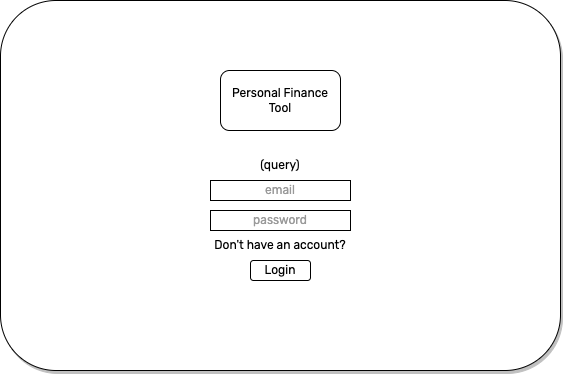
\includegraphics[width=0.7\textwidth]{images/Login_specification.png}
	\caption{Login Page}
	\label{fig:LoginPage}
\end{figure}

Above is the basic design for these pages. Most of it is self explanatory, however where it says "(query)" is where any message or response can be displayed to the user. These include "you have successfully logged out", or "that user does not exist", or "incorrect password", and will be given the relevant colours . The "don't have an account?" and "login" text will be modified appropriately for each page that it is on - for example if instead the user is creating an account, it will say "already have an account?" and "signup" respectively.

This was the first and only page that was styled from a draw.io specification as the process of doing this was found quite slow and tedious. It didn't maximise the value of using TailwindCSS to quickly add the CSS classes and perform dynamic styling. For the rest of the pages, the more efficient process outlined in the introduction to this section was followed.

\subsection{Dashboard}
Once the minimum strategies for the web application had been determined - transactions, categories, budgets and investments. It was decided that this information was to be presented on a single central page, and the ability to switch between the strategies is done via a header bar. The was so quick access to all the information is possible, but also so that strategies not being viewed can be preloaded in the background to avoid long waits for the information to load, ultimately improving the user experience.

\begin{figure}[h!]
	\centering
	
\includegraphics[width=\textwidth]{images/Header_nav_bar.png}
	\caption{Dashboard Navigation Bar}
	\label{fig:DashboardNavigationBar}
\end{figure}

The header bar shown above (\ref{fig:DashboardNavigationBar}) was initial design for this dashboard (and minimally changed in the final product). By default, the transactions strategy is chosen. When hovering on the other strategies, a light grey bar underneath the strategy name appears; then being selected turns this bar orange and removes the bar from the old strategy. Underneath this bar is the information provided for that strategy, for example in the transactions strategy, below will be all the transactions.

A limitation in the current systems that was outlined earlier is the ability to include several accounts. Furthermore, of the few that do have this feature, none of them have a way to easily enable/disable the incorporation of these accounts in the analytics. Therefore, this aspect was key when thinking about the design of the header bar. On the right in a slightly different bar, there is an accounts dropdown. When clicking on this, all the bank accounts that the user as linked will be displayed hear, along with a toggle button to enable/disable the account. Only enabled accounts will be included in the analytics, and when switching between strategies, only the selected accounts will persist. An ideal use case for this feature is when a user has several accounts, but only wants to see their transactions on their savings accounts. They can disable all the other accounts to do so. Following this, they can quickly re-enable the other accounts when they want to see them all again by just clicking the toggle button.

\section{Strategies}
The only pages in the whole application are the two described above (authentication and dashboard). Each of the strategies will be implemented as separate components but will appear on the dashboard page. This means that each component ought to be roughly styled in the same way as to match the general theme.

\subsection{Transactions}
This is the default strategy that is shown on the dashboard because it contains the information that would be the most useful in helping the user can an overview of their finances. By viewing their recent transactions, they can see where money is being spent and where it is coming from, and then make adjustments accordingly. A lot of traditional banks to not allow quick access to this information, and viewing transactions for all the accounts that have been toggled on can be extremely useful in identifying expenses that are not necessary.

From Plaid, the endpoint returns a list of transactions in reverse chronological order, per account. Each transaction has account\_id, amount, date, time, location, currency code, merchant name, category and more. The web application will group the transactions from all toggled accounts by their date, then display each transaction in reverse chronological order. The transaction will be displayed with the merchant name, category, amount and the bank logo of the account it is from. For each date their will be a separate label above all the transactions for that date. Finally a distinction between income and expenditure will be made by colouring the whole transaction background light-green for income and light-red for expenditure.

\begin{figure}[h!]
	\centering
	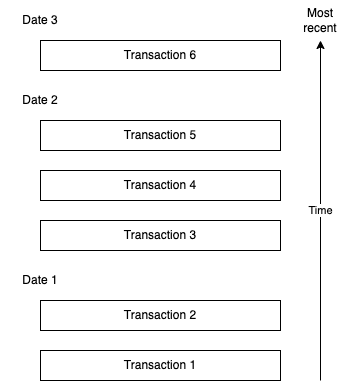
\includegraphics[width=0.6\textwidth]{images/Transaction_labels.png}
	\caption{Reverse Chronological and Date Grouped of Transactions}
	\label{fig:TransactionLabels}
\end{figure}

\subsection{Categories}
The categories strategy would also be helpful at identifying unnecessary expenses. In this case, the application only takes the previous thirty days, and also only takes expenditure. It will list all the transactions in reverse chronological order again, but this time not grouped by anything. A pie chart will also be displayed with the values being the total amounts for each category. The user can then see which category they are spending the most in, and will be able to see the total amounts. In addition, they will be able to group each transaction by it's category and show only the transactions for that category by selecting it. All the transaction data will again be only for the toggled accounts.

The difference between this strategy and the transactions strategy is that in the transaction strategy, the emphasis will be on if the transactions were income or expenditure and to which back account; whereas in teh categories strategy, the emphasis will be on the category of the transaction and the total amount spent in that category. The input data will be the same, but it is a different way of presenting the data such that the user can get all the perspectives on their finances, and ultimately make better decisions.

\subsection{Budgets}
Two different methods of performing some analytics of budgets were considered for this strategy. The first method was giving the user a budget breakdown based on their income. Following some research, it was found that for the average person, utilising a 50:30:20 budget is extremely effective at helping people spend money on the necessities, still having some money for treats and also saving some money. The article \cite{503020Strategy} by N26, a well respected european bank, explains the strategy in more detail. In essence, it says to spend 50\% of your income on needs, 30\% of your income on wants, and 20\% of your income into savings. Several other articles back up the effectiveness of this strategy and help give it credibility; \cite{503020InCostLivingCrisis} even talks about how this method carries over into the cost of living crisis. 

The method does have some disadvantages however. The major one being that it is extremely difficult to narrow down which category each expense falls under. Often people will disagree what is considered essential, so is already subjective. A common example found from some of the articles that talk about it is a gym membership. In addition, altering your spending habit is quite difficult and often if your income is relatively low, it may not even be possible to save 20\% of your income.

The design for this strategy would be to have an input element where the user can enter their income, however it would also help determine the income from previous transactions. The website would then breakdown their income into the 3 sections and give them values for what they can spend on each. Finally, for their previous thirty days of transactions (the usual time period between each pay day), the user will be able to drag and drop each transaction into the three categories to help them see how much they are currently spending. If they are spending too much on any, they can make adjustments accordingly.

The other method that was considered for a budgeting strategy was to perform budget prediction. This would involve viewing how much they have spent so far for the current month, and performing some pattern recognition to make predictions for the remaining days. They could then compare this to a budgeted amount they planned to spend that month and identify if they are on track. This would be useful for people who are trying to save money for a specific goal, such as a holiday or a new car. The user would be able to see if they are on track to reach their goal, and if not, they can make adjustments to their spending habits to reach it.

The method of performing the prediction can vary from manual pattern identification to machine learning, so at this stage it was more relevant to identify which strategy would be most effective as performing the original aim of the project. Overall, the budget prediction method was more appropriate because every use could utilise the information it provided, furthermore, it also provided analytics which would be extremely difficult for the user to manually, unlike the 50:30:20 method. Also in predicting future expenses, the user could make adjustments to what they spend money on sooner, before it becomes a problem so is more effective.

\subsection{Investments}
According to Finder.com, a reputable source for financial information, in Danny's article on investment statistics, he says that "Almost 1 in 5 Brits have owned stocks or shares" \cite{InvestmentStats}. This is from a survery completed in the year 2023, so is recent, and is fact checked by other journalists. With over 13 million people in britain alone, a strategy to adhere to this demographic would be useful and popular.

A particularly useful tool, which continues the idea of getting an overview of the user's finances, would be a central portfolio manager where logged in users can view and track their investments. This would be the only strategy that doesn't utilise Plaid to access the data, so instead the user would have to add it themselves; however, this is not a problem as unlike the other strategies, once the asset had been purchased, they would only need to add it once. Following this, every time the user would come to check their investments, they could see the updated live price and view the amount of profit or loss they have made.

In order to perform this strategy, once the user has added their investments, they need to be stored. One option would be to store them in local storage within the browser. This would be the simplest to implement and as stored offline, would be somewhat secure, however it would have some disadvantages. To begin with, it would only be accessible from the same device and browser, so if the user wanted to access the tool from another device, they would have to add them again. In addition, if the user cleared their browser data, they would lose the investment entry so also have to manually add it again.

The other option would be to persist them using a database. As a PocketBase data store is already being used for the application, this wouldn't require too much extra work and complexity; furthermore, there are some major advantages. Unlike local storage, when using the database, the information is accessible and up to date from any device or browser, so the investment would only have to be added once. Also by linking the investments to only be accessed by the user who created them, they would be extremely secure and could be treated like the Plaid access\_tokens.

In the end, the database option was chosen because synergises well with the current design of the system and has the same advantages as local storage. As well persisting the investments, the application would also have to get the current price of the investment to determine if is profitable. To do this, the application would have to make a request to a service that provides the current price of the investment. Financial modelling prep is an easy to use service that provides quick and live stock prices so is ideal for this task. Given the price the investment was bought for, and the current price, the application would be able to calculate the profit and for example could be displayed as green for positive, and red for negative. This means the user can identify which investments are profitable and should continue, as well as which ones are not and action should be taken. 

\section{Budget Prediction}
One decided that budget prediction was the method for the budgeting strategy, the actual prediction method needed to be designed. For this there was 3 different considerations: a basic manual pattern identification method; utilising linear regression to find the relationship; and using a neural network to find the trends. For each of the method, the only accessible real training data was the author's past 3 years of transactions, so this factor has to also be considered when deciding which method to use.

\subsection{Manual Pattern Identification}
This method would be the simplest to implement and would involve manually identifying the patterns. Given the training data, set time periods would be suggested and then determining which one and by how much is the biggest of these. For example, given the three years transactions, split the data into the different seasons and identify in which season is the most spent. Using this knowledge, if a query is wanting a prediction in the most expensive season, then increase the normal prediction. This can be repeated on many different features, each of different time periods such as weeks, weekends, months, national holidays. Once many different factors have been analysed, the prediction can be made by combining all the factors together. This method would be very fast at making a prediction, but extremely complicated and inaccurate to initially implement. Furthermore, the predictions may not be very accurate as some features may not be factors, and others may not have been considered. Ultimately, this method would sacrifice accuracy for speed and complexity.

\subsection{Linear Regression}
Linear regression is a method for "modelling the relationship between a scalar response and one or more explanatory variables" \cite{LinearRegressionWiki}. To apply it to budget prediction, the output expenditure would be the scalar response, and the explanatory variables would include the budget set out by the user as well as the current date. The model would find the relationship based on the past 3 years of data, and then when a query comes in, it would quickly be able to use the learnt relationship to output an expected expenditure. The main advantage of this method is that it would not involve any manual pattern identification and the relationship would be computed. Despite this, it still wouldn't be that accurate as the relationship between expenditure and explanatory variables almost definitely will not be linear, which is the major downfall. One option to counter this would be to project the input data into a higher dimension. This would allow the model to find linear relationship in this projected space, but then a better non-linear relationship in the original space. This would be a good option, but would require a lot of computation to do so, may be considered over engineering for this problem, and would not even guarantee a better result.

\subsection{Neural Network}
The final option that was considered was to use a neural network. This would take the input data, manually identify the features and trends and then, with lots of training data, learn the patterns. Within choosing to do a neural network, there is still so much variation as each model can be very different. The neurons themselves can have different activation functions, but also the connections between them. It can be feed-forward with no loops or be a recurrent neural network with some feedback. Each layer can have various number of neurons and the number of layers can also vary. Acknowledging this, if the network was to be designed effectively, it could out perform the other two methods in terms of accuracy so would be most ideal for this problem. The drawbacks include the fact that it would involve a lot of testing and tuning to get the best results, and the fact that the input data is limited doesn't help.

\subsection{Conclusion}
In the end, out of the three options described above, the most applicable model for the problem of budget prediction was a neural network. This was because it didn't rely on manually finding the features to use, so would identify even the hidden and complex patterns, as well as, after being trained, generate quick predictions with high accuracy. The implementation of the budget prediction is described in much more detail in the implementation section \ref{ch:implementation}, but a quick overall explanation is given below.

Deciding the architecture of the neural network would involve lots of trial and error to identify what is most appropriate. There is little research on the topic of predicting expenditure given past expenditure so not much even to help start. Through generalising the problem, the key idea which helped was to think of the problem as a time series problem. By modifying the input data from being a list of chronological transactions, to instead being the cumulative amount spent each day and resetting every month, the input data could be treated as a time series. This has much more research as a problem because time series prediction is a very important area for many industries, such as trading companies trying to predict the stock market. Applying lots of these ideas that have been applied to time series data found that using a recurrent neural network was the most effective.

\section{Software Architecture}

\begin{figure}[H]
	\centering
	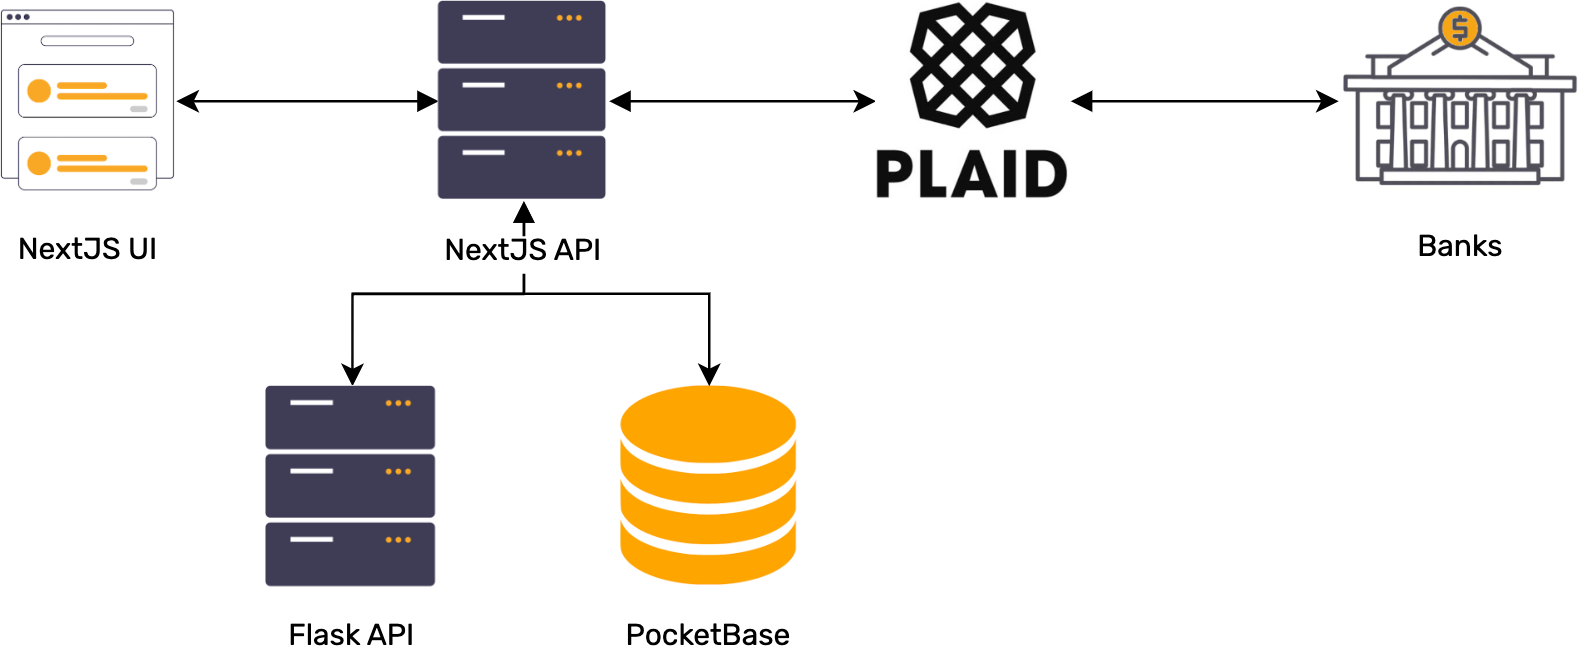
\includegraphics[width=\textwidth]{images/Architecture.drawio.png}
	\caption{Software Architecture}
	\label{fig:SoftwareArchitecture}
\end{figure}

The figure above (\ref{fig:SoftwareArchitecture}) shows the software architecture of the project and the interactions between each service. The four on the left have been developed as part of this project, with the two on the right pre-existing entities. The user interacts with the front end, which is the Next.js UI. Having this separation from the backend was required for the Plaid authentication. The Next.js API routes are how the UI communicates with Plaid and the database. An example API route would be "get\_transactions", where the backend then returns the transactions received from Plaid, which itself returns the transactions from the bank itself. The access\_tokens and other long-term information such as user's login details are stored in the PocketBase database. This can only be accessed by the backend, and for example the access\_tokens can only be accessed by the user's who created in them in the first place for extra security. Finally, there is the Python Flask API which contains the budget prediction neural network. This API only has one route, which takes in the input data, propagates its through the neural network, and returns the output. It must be queried by the Next.js API routes as the input data requires the user's path month's transactions, therefore they must be requested from Plaid. This means when the Budget prediction page is accessed, the frontend queries Next.js, which itself queries the Python Flask API, after retrieving the transactions from Plaid. The Python Flask API then returns the prediction to the Next.js API, which then returns it to the frontend to be displayed.

\section{Endpoints}
\label{sec:endpoints}
Given the design for the strategies that the web application will exhibit, various Next.js API routes will be required. All of these routes will be prefixed with "/api" to be accessed by the client, and will be accessed using the HTTP POST method. This is because the requests often need to contain some contextual information for the server to decide what to do, for example, contain the user identifier to determine which user's transactions are being requested. The information passed between the client and server will be in JSON format as helps represent the data in a structured format as well as being easy to parse by both the client and server being written in JavaScript. In addition, python has a built in JSON library to work when communicating with the Python Flask API. Also each route will be written such that it can only perform its intended function or return an error. This is such that all the error checking can be done on the client side to improve security, as well as reduce the amount of code to be written and make the user experience better for graceful error handling.

\section{Legal, Ethical and Professional Considerations}




